\subchapter{Interacting with the Networking Stack}
{Objective: learn how to manage Networking interfaces and create new ones}

\section{Goals}

\begin{itemize}
\item Get familiar with the Espressobin's network interfaces
\item Use \code{iproute2} for link configuration, vlan setup and bridiging
\item Use the different VLAN configuration methods
\item Use network namespaces for interface isolation
\end{itemize}

\section{Getting familiar with the Espressobin}

The Espressobin has 3 front-facing ports labelled "wan", "lan0" and "lan1" :

\begin{center}
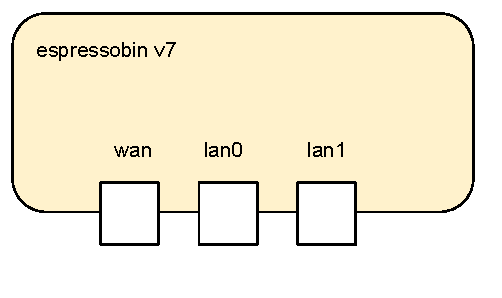
\includegraphics[width=0.5\textwidth]{labs/networking-stack/01_LAB1_espressobin.pdf}
\end{center}

List the network interfaces by running :

\begin{targetbashinput}
$ ip link show
\end{targetbashinput}

Do you notice anything strange ? Besides the \code{lo} interface for loopback,
we see 4 interfaces :

\begin{itemize}
\item \code{eth0}
\item \code{lan0@eth0}
\item \code{lan1@eth0}
\item \code{wan@eth0}.
\end{itemize}

This is because the Espressobin uses a dedicated \textbf{DSA switch} to drive its ports,
and \code{eth0} is used as conduit between the \textbf{SoC's Ethernet Interface} and one of the switch's ports.

In this lab, we will ignore \code{eth0} and only focus on the other 3 interfaces.
Although they appear as \code{lan0@eth0}, you must use the shorter \code{lan0} interface name in your commands.

\newpage

\section{Sending our first packet}

Let's send out first ping between our Host machine and the Espressobin. This is the setup we'll achieve :

\begin{center}
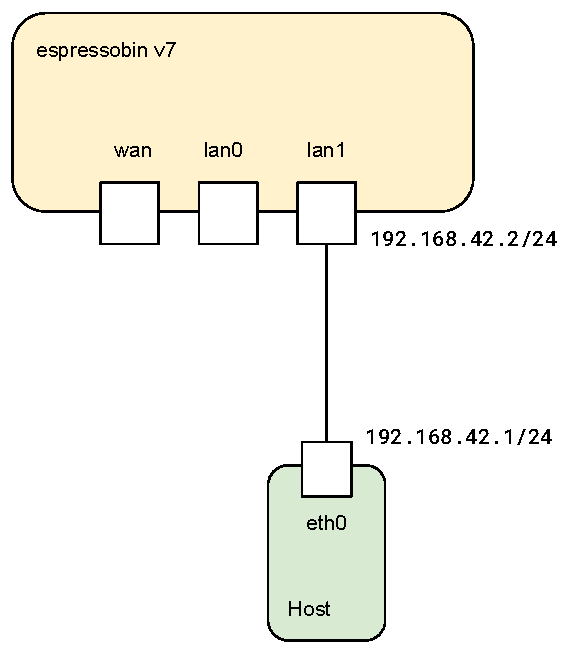
\includegraphics[width=0.5\textwidth]{labs/networking-stack/02_LAB1_espressobin_1to1.pdf}
\end{center}

The first step we need to take is to administratively bring the \code{lan1} interface \textbf{up} :

\begin{targetbashinput}
$ ip link set lan1 up
\end{targetbashinput}

You can check that an interface is "admin UP" by running :


\begin{targetbashinput}
$ ip link show lan1
3: lan1@eth0: <NO-CARRIER,BROADCAST,MULTICAST,UP> ...
\end{targetbashinput}


The "UP" keywork appears as the last element betweek the chevrons following the interface
name, this is the admin link state. When the interface is "admin down", no keywork will appear in that spot.

The next step is to check that we have a working connection with the Host. Plug the Ethernet cable between the \code{lan1} port
and your Host machine. Make sure that your Host's interface is UP as well. Let's check the link status one more time :

\begin{targetbashinput}
$ ip link show lan1
lan1@eth0: <BROADCAST,MULTICAST,UP,LOWER_UP> mtu 1500 qdisc noqueue state UP ...
\end{targetbashinput}

The \code{LOWER_UP} indication tells you that there's a \textbf{link-partner} detected, using \textbf{PHY Layer} information when available.
The \code{state UP} keywords indicates that the whole link between this interface and the link partner is up and running, ready to transmit traffic.

\newpage

To get information about the PHY layer attributes, you can use \textbf{ethtool} :

\begin{targetbashinput}
$ ethtool lan1
\end{targetbashinput}

\begin{targetterminaloutput}
Settings for lan1:
	Supported ports: [ TP	 MII ]
	Supported link modes:   10baseT/Half 10baseT/Full
	                        100baseT/Half 100baseT/Full
	                        1000baseT/Full
	Supported pause frame use: Symmetric
	Supports auto-negotiation: Yes
	Supported FEC modes: Not reported
	Advertised link modes:  10baseT/Half 10baseT/Full
	                        100baseT/Half 100baseT/Full
	                        1000baseT/Full
	Advertised pause frame use: Symmetric
	Advertised auto-negotiation: Yes
	Advertised FEC modes: Not reported
	Link partner advertised link modes:  10baseT/Half 10baseT/Full
	                                     100baseT/Half 100baseT/Full
	                                     1000baseT/Full
	Link partner advertised pause frame use: Symmetric Receive-only
	Link partner advertised auto-negotiation: Yes
	Link partner advertised FEC modes: Not reported
	Speed: 1000Mb/s
	Duplex: Full
	Auto-negotiation: on
	Port: Twisted Pair
	PHYAD: 17
	Transceiver: external
	MDI-X: Unknown
	Supports Wake-on: d
	Wake-on: d
	Link detected: yes
\end{targetterminaloutput}

We can get from the above that : 
\begin{itemize}
\item The link is \textbf{up} : \code{Link detected: yes}
\item The link speed was established at 1Gbps : \code{Speed: 1000Mb/s}
\item The Link-partner (Host machine) supports 10, 100 and 1000Mbps links
\end{itemize}

To send our first ping, we now need to assign IPv4 addresses to both \code{lan1} as well as our Host's interface. Let's use the \code{192.168.42.0/24} subnet :

\begin{targetbashinput}
$ ip address add 192.168.42.2/24 dev lan1
\end{targetbashinput}

You can show the currently assigned IP addresses to each interface by running :

\begin{targetbashinput}
$ ip address
\end{targetbashinput}

Run a similar command on your host machine to assign it the \code{192.168.42.1/24} address.

You can now send your first \textbf{ping}, running the following command on your Host machine :

\begin{hostbashinput}
$ ping 192.168.42.2
\end{hostbashinput}

\section{Create a VLAN}

Now that we know that the link between our Host machine and the Espressobin works,
let's setup a VLAN link.

First, remove any prior IPv4 configuration we've done on \code{lan1} :

\begin{targetbashinput}
$ ip address flush lan1
\end{targetbashinput}

The setup we want to achieve is the following :

\begin{center}
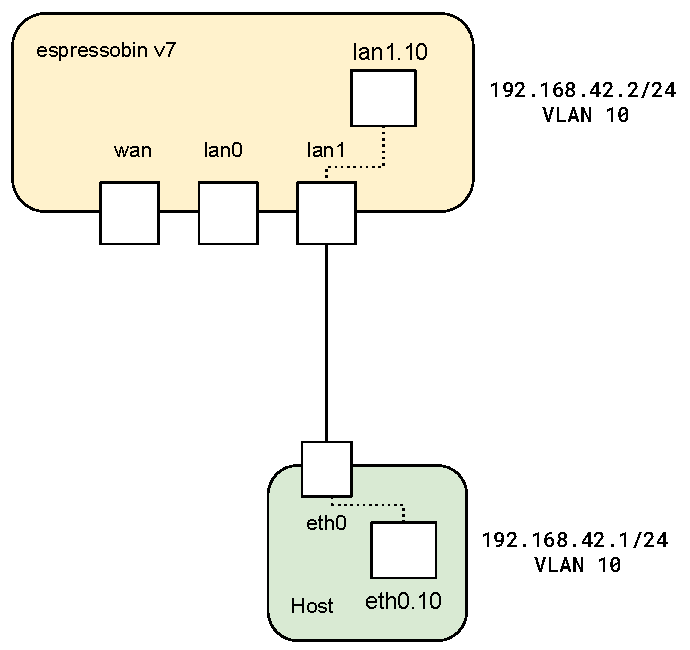
\includegraphics[width=0.5\textwidth]{labs/networking-stack/03_LAB1_espressobin_vlan.pdf}
\end{center}

We'll use a dedicated netdevice for the VLAN we want to create. We will use VLAN id 10, which is arbitrary here. We assign an IP address to the vlan interface, and set it as admin-up :

\begin{targetbashinput}
$ ip link add link lan1 name lan1.10 type vlan id 10
$ ip address add 192.168.42.2/24 dev lan1.10
$ ip link set lan1.10 up
\end{targetbashinput}

Configure your Host machine in the same way, with the same VLAN id, but adjusting the IP address.

You should now be able to ping your Espressobin from your Host. Leave the \code{ping} command running, we'll need some traffic to go through for this next part.

Let's go a bit further and capture some traffic, to see what the encapsulation looks like. For now, we'll only use \code{tcpdump} as our capturing software.

\begin{targetbashinput}
$ tcpdump -n -e -i lan1.10
\end{targetbashinput}

You should see the ICMP traffic generated by the \code{ping} command running on your host :

\begin{targetterminaloutput}
[...] ethertype IPv4 (0x0800), length 98: 192.168.42.1 > 192.168.42.2: ICMP echo request, ...
[...] ethertype IPv4 (0x0800), length 98: 192.168.42.2 > 192.168.42.1: ICMP echo reply, ...
[...] ethertype IPv4 (0x0800), length 98: 192.168.42.1 > 192.168.42.2: ICMP echo request, ...
[...] ethertype IPv4 (0x0800), length 98: 192.168.42.2 > 192.168.42.1: ICMP echo reply, ...
\end{targetterminaloutput}

Traffic captured on \code{lan1.10} doesn't show any VLAN tag, as this interface will expose \textbf{untagged} traffic to the user.

\newpage

Exit \code{tcpdump} with \code{ctrl-c}, and now dump the traffic going through \code{lan1} :

\begin{targetbashinput}
$ tcpdump -n -e -i lan1
\end{targetbashinput}

\begin{targetterminaloutput}
[...] ethertype 802.1Q (0x8100), length 102: vlan 10, p 0, ethertype IPv4 (0x0800), 192.168.42.1 ...
[...] ethertype 802.1Q (0x8100), length 102: vlan 10, p 0, ethertype IPv4 (0x0800), 192.168.42.2 ...
[...] ethertype 802.1Q (0x8100), length 102: vlan 10, p 0, ethertype IPv4 (0x0800), 192.168.42.1 ...
[...] ethertype 802.1Q (0x8100), length 102: vlan 10, p 0, ethertype IPv4 (0x0800), 192.168.42.2 ...
\end{targetterminaloutput}

You can now notice that traffic going through \code{lan1} contains a \textbf{802.1Q} tag with the VLAN id of \code{10}. The frames are also 4-bytes longer, which corresponds to the length of a 802.1Q tag.

\section{Looping back}

Let's take a step back from VLANs for now, and focus on the other interfaces of the espressobin.
Clean-up the previous part's setup by removing the vlan interface :

\begin{targetbashinput}
$ ip link del lan1.10
\end{targetbashinput}

We'll try to perform a simple test by looping back the \code{wan} and \code{lan0} interface :

\begin{center}
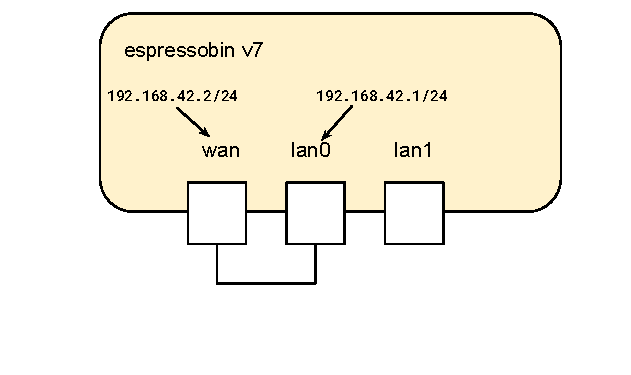
\includegraphics[width=0.8\textwidth]{labs/networking-stack/04_LAB1_espressobin_loopback.pdf}
\end{center}

Connect \code{wan} and \code{lan0} together with one of the provided Ethernet cables, and configure both
interfaces with the \code{ip} command, using the addresses indicated in the above schematic.

Check that your link parameters are sensible with \code{ethtool}, and that you can send simple ICMP traffic with \code{ping}.

You will see the ping command working. However, we are pinging a local address, so make sure there's traffic flowing through our loopback cable. One of the ways
of checking this is to looks at the \textbf{hardware counters} exposed by our drivers. This is done with \code{ethtool -S <iface>} :

\begin{targetbashinput}
$ ethtool -S wan | grep tx_packets
\end{targetbashinput}

Check that this counter increments when sending traffic with \code{ping}.

As you may have guessed, the counters aren't incrementing although we do see the ping
going through. This is because the Linux Kernel sees we're pinging a local addresses, and responds to it
without involving our hardware interfaces.

To circumvent that, let's use \textbf{Network Namespaces} to isolate our interfaces from one another :

\begin{center}
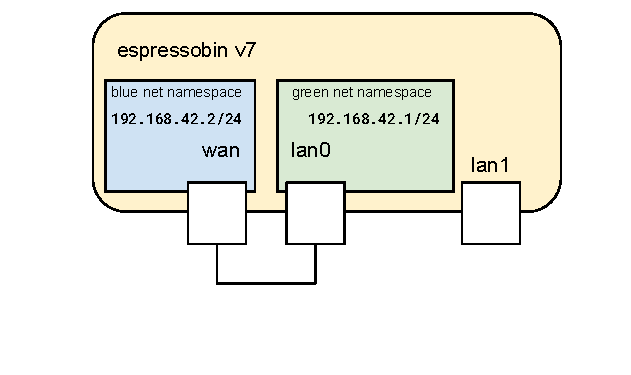
\includegraphics[width=0.8\textwidth]{labs/networking-stack/05_LAB1_espressobin_loopback_netns.pdf}
\end{center}

We'll use the \code{blue} netns for the \code{wan} interface, and the \code{green} netns for \code{lan0} :

\begin{targetbashinput}
$ ip netns add blue
$ ip link set dev wan netns blue

$ ip netns add green
$ ip link set dev lan0 netns green
\end{targetbashinput}

From that point on, you will no longer see the \code{wan} and \code{lan0} interfaces when running \code{ip link show}, as they are no longer in the \textbf{init namespace}. To interact with them, you need to execute the commands within the namespace :

\code{ip netns exec green <cmd>}

You will now need to re-configure each interface, as they were flushed when entering the new namespace :

\begin{targetbashinput}
$ ip netns exec blue ip link set wan up
$ ip netns exec blue ip address add 192.168.42.2/24 dev wan

$ ip netns exec green ip link set lan0 up
$ ip netns exec green ip address add 192.168.42.1/24 dev lan0
\end{targetbashinput}

Now, try to ping one the \code{wan} interface from the \code{green} namespace :

\begin{targetbashinput}
$ ip netns exec green ping 192.168.42.2
\end{targetbashinput}

Check that the counters on \code{wan} are incrementing :

\begin{targetbashinput}
$ ip netns exec blue ethtool -S wan | grep tx_packets
\end{targetbashinput}

\section{Bridging}

Let's continue our quest to have the most convoluted setup with our espressobin.

We'll re-use what we have configured so-far with our namespaces, let's just flush the IP address from \code{lan0} :

\begin{targetbashinput}
$ ip netns exec green ip address flush lan0
\end{targetbashinput}

We will create a \textbf{bridge} \code{lan0} and \code{lan1} so that we can use them as ports of a same \textbf{switch} :

\begin{center}
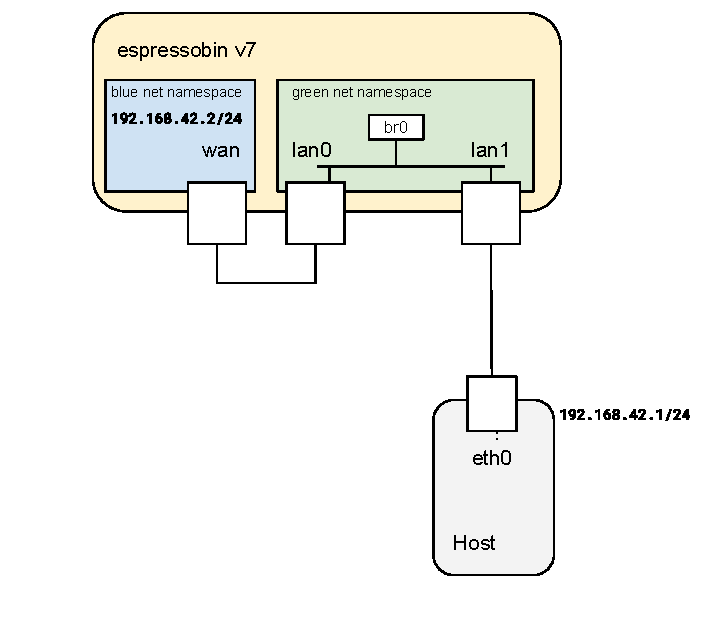
\includegraphics[width=0.5\textwidth]{labs/networking-stack/06_LAB1_espressobin_bridge.pdf}
\end{center}

First, let's create a new bridge device (in the green netns) :

\begin{targetbashinput}
$ ip netns exec green ip link add name br0 type bridge
$ ip netns exec green ip link set br0 up
\end{targetbashinput}

Next, let's add \code{lan1} to the green netns :

\begin{targetbashinput}
$ ip link set lan1 netns green
$ ip netns exec green ip link set lan1 up
\end{targetbashinput}

Finally, add both \code{lan0} and \code{lan1} to the bridge :

\begin{targetbashinput}
$ ip netns exec green ip link set dev lan0 master br0
$ ip netns exec green ip link set dev lan1 master br0
\end{targetbashinput}

Make sure your Host's IP address is \code{192.168.42.2/24}, then try to ping it !

Congratulations !
